\section{Preliminaries}

\subsection{Concepts}
\begin{figure}[t!]
\centering
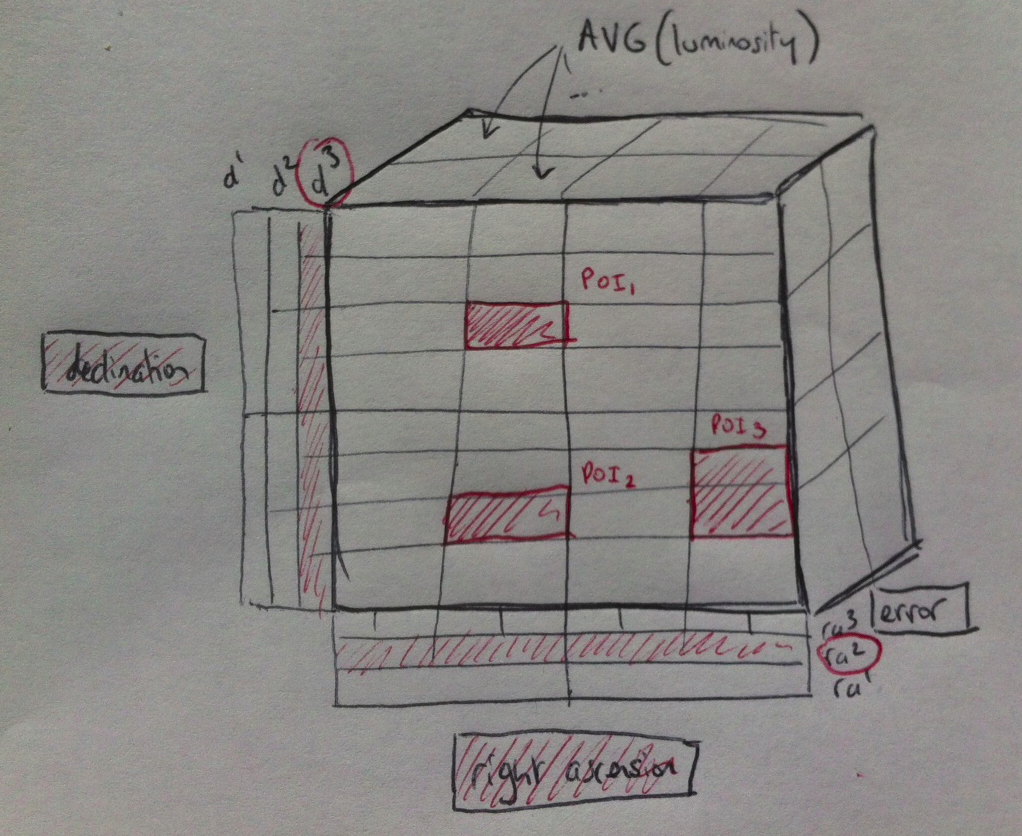
\includegraphics[width=0.9\columnwidth]{images/cube}
\caption{Example of recommendation}
\label{cube}
\end{figure}
We model the database as a large relation $DB$. This table contains two types
of columns: the dimensions $D_0, \ldots, D_d$ and a target column $T$. The
target column contains the target value for each tuple. Note that this view is
logical: we are oblivious to the physical structure of the data.  Claude's aim
is to generate a set of \textbf{explanations}.  An explanation contains two
elements: a \textbf{view} and several \textbf{points of interest} (POI). A view
is an ``informative'' set of dimensions, on which we project the data.  A point of
interest is a selection over this view. It contains tuples for which the target
has a ``remarkable'' distribution.

We illustrate these concepts with Figure \ref{cube}. Our example database
describes light sources.  It contains three dimensions: \texttt{right
ascension}, \texttt{declination} and \texttt{error}. The first two describe a
source's position. The third one describes the measurement errors. For each
tuple, we target the value of the column \texttt{brightness}. Claude's output
is highlighted in red. It contains a view based on \texttt{right ascension},
and \texttt{declination}. We see that the view is a SQL query with the
following structure:
\begin{verbatim}
SELECT   D1, ... , Dn , AVG(T)
FROM     DB 
GROUPBY  D1, ... , Dn
\end{verbatim}
The $n$ distinct variables $\texttt{D1} \ldots \texttt{Dn}$ define the view. Once
Claude has chosen a view, it must explain \emph{why} it has chosen this view.
This is the role of POIs. In Figure \ref{cube}, Claude suggests four POIs. We
can express them in SQL as follows:
\begin{verbatim}
SELECT   AVG(T)
FROM     DB
WHERE    D1 BETWEEN l1 AND h1
 AND     ...
 AND     Dn BETWEEN ln AND ln
\end{verbatim}
The POIs are defined by the ranges $\texttt{[l1,h1]}, \dots \texttt{[ln,hn]}$.


\subsection{Informative explanations}
\label{sec:infor}
\begin{figure}[t!]
\centering
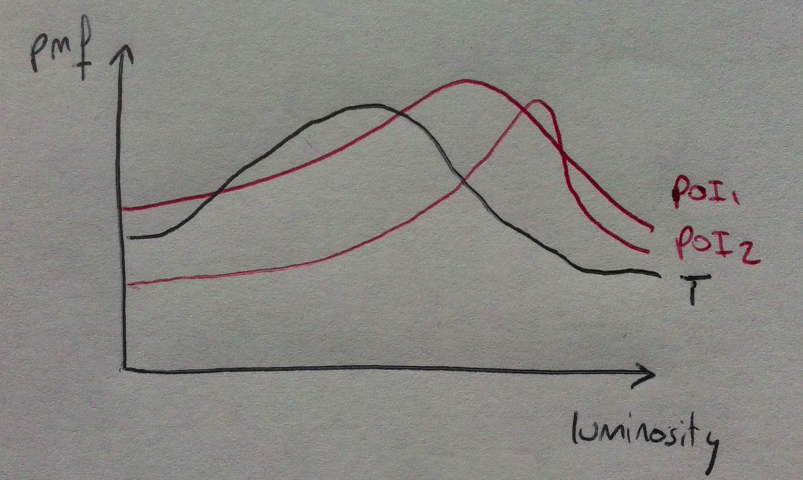
\includegraphics[width=\columnwidth]{images/poi}
\caption{The POIs have unusual distributions}
\label{poi}
\end{figure}

We defined Claude's search space: we want to suggest views and POIs. We now
present how the target helps us recognize the ``interesting'' ones. 

First let's explain how to choose the views. A set of columns is informative if
it is somehow related to the target: if we filter the data on these columns, the target
value changes.  We model this relationship with statistical dependency. We
represent each  dimension $D_k$ by a random variable $\rv{D}_k$. We model the
target with a random variable $\rv{T}$.  A view is interesting if there exists
some statistical dependency between its columns and the target. We formalize
this statement with Mutual Information \cite{cover2012elements}:

\begin{definition}
Consider a view $V = \{D_1, \ldots, D_n\}$, and the target column $T$.  Let
$I$ denote the \emph{Mutual Information} between two random variables. We
define the \textbf{strength} of $V$ as follows:
\[\sigma(V) = I(\rv{D}_1, \ldots, \rv{D}_n ; \rv{T})\]
\end{definition}

Claude seeks variables which are jointly related to the target. Note that it
considers any kind of statistical relationship, not only correlation.
The next step is to extract the POIs. The POIs contain tuples for which the
measure have an ``unusual'' distribution compared to the rest of the database.
Consider Figure \ref{poi}. The curves show the probability mass function of the
brightness for three sets of tuples: the whole database, $POI_1$ and $POI_2$.
The sets $POI_1$ and $POI_2$ come from the view \texttt{right ascension -
declination} in Figure \ref{cube}. We observe that they deviate from $DB$.
They illustrate how right ascension and declination can influence
brightness. We quantify this observation with the Kullback-Leibler
divergence:

\begin{definition}
Consider a range $R = [l_1, h_1] \times \ldots \times [l_n, h_n]$. 
The random variable $\rv{T}_R$ describes the target for
the tuples in $R$, and $\Pr(\rv{T}_R)$ its distribution.
We define the \textbf{divergence} of the range $R$ as follows: 
\[\delta(R) = KL \big( \Pr(\rv{T}_R) \| \Pr(\rv{T})  \big)\]
\end{definition}

The Kullback-Leibler divergence measures the difference between two probability
distributions. Our function $\delta$ grows when a range has unsual target
values, it decreases otherwise. It does not target specifically high or low
values. It seeks \emph{any} type of deviation from the target's global distribution.
Note that divergence is tightly related to strength:

\begin{lemma}
Let $V$ denote a view. We discretize each variable. The variable $\rv{R}$
describes a random bin.  We observe the following relationship:
\[
    \sigma(V) = \mathbb{E}_{\rv{R}} \{ \delta(\rv{R}) \}
\]
\end{lemma}

\begin{proof}
Let $\rv{V}$ represent the joint distribution $\rv{D}_1, \ldots, \rv{D}_n$.
We have $\sigma(V) = I(\rv{V},\rv{T})$.
By definition of the Kullback-Leibler divergence, we have: 
$I(\rv{V},\rv{T}) = $ $\mathbb{E}_{\rv{V}} \{ KL( \Pr(\rv{T} | \rv{V}) \|$ $ \Pr(\rv{T}) ) \}$
As the data is discretized, $\rv{V}$ and $\rv{R}$ are equivalent. Also,
for any bin $R$, $\Pr(\rv{T} | \rv{V} = R)$ is equivalent to
$\Pr(\rv{T}_R)$. We derive the lemma.
\end{proof}


This lemma is simple but powerful. It shows that strength and divergence are
``two sides of the same coin'': the strength of a view equals exactly the
average divergence of its bins. We use the terms strength and
deviation interchangeably to characterize an \emph{explanation} (recall that a
explanation contains both the view and its POIs).

\begin{definition}
Let $S=(\{ D_1, \ldots, D_n\}, \{R_1, \ldots, R_r\})$ describe an explanation . The
\textbf{strength} (or \textbf{divergence}) of $S$ equals the strength
of its view.
\end{definition}

We are now ready to formulate our problem.

\begin{problem}
Consider a hypercube $DB$, a target column $T$ and a triplet $(q, n, r)$. Find
the top $q$ strongest explanations, with $n$ variables and $r$ POIs.
\end{problem}

To solve this problem, Claude operates in two steps. First, it detects $q$
strong sets of columns.  We call this step \emph{column search}.  Then comes
the \emph{POI dectection} step: for each view we extract $r$ POIs. In practice,
our top $q$ strategy can generate redundancy. We tackle this problem with an
optional \emph{refinment} step.

\section{Column selection}
\label{sec:colum}

The aim of this phase is identify the $q$ strongest sets of variables. From
here on, we use the notations $D_i$ and $\rv{D}_i$ interchangeably. We can use
the context to distinguish database columns and random variables.

\subsection{Base algorithm}

\begin{figure}[t!]
\centering
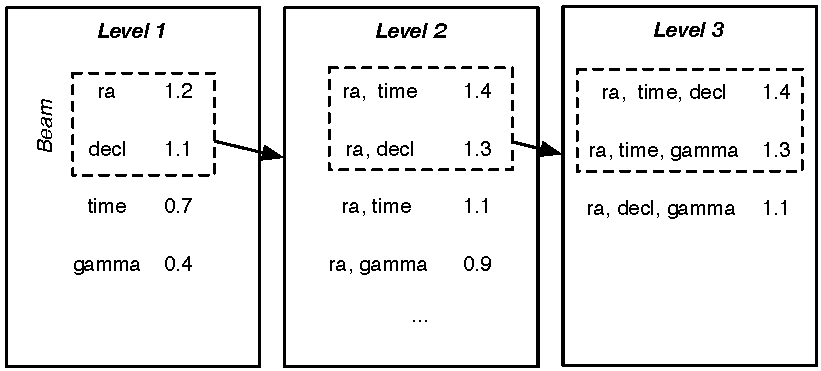
\includegraphics[width=0.8\columnwidth]{images/beam-search}
\caption{Example of Beam Search, with a beam size of 2}
\label{pic:beam-search}
\end{figure}

To recommend views, Claude must find the best sets of at most $n$ variables.
The search space of this problen grows exponentially with $n$: from a database
with $d$ variable, we can generate $\sum_{i \leq n} \binom{d}{i}$ combinations.
Besides, there is to our knowledge no bound which would allow us to prune the
search space efficiently. Therefore, we use level-wise search. To initialise
the algorithm, we compute the strength of each variable in isolation.  To do
so, we compute the mutual information between the target $T$ and each dimension
$D_i$, $\sigma(D_i) =  I(D_i; T)$. We order the candidates, and keep the top
$b$ results. We call this set the \emph{beam}. We then form new candidates by
appending each variable of the database to each view in the beam. We compute
the best $b$ results and update the beam. The procedure is repeated until the
beam contains views with $n$ variables. We illustrate the procedure in Figure
\ref{pic:beam-search}.

\begin{figure}[t!]
\centering
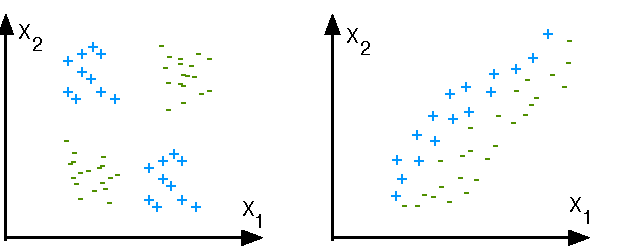
\includegraphics[width=0.8\columnwidth]{images/strength-jump}
\caption{Limit cases of the beam search strategy. The variables $var1$ and
$var2$ represent two dimensions. The symbol and color of the plots represent
the value of the target class. }
\label{pic:strength-jump}
\end{figure}
Thanks to our beam strategy, we avoid exploring an exponentially large search
space. Instead, we compute the strengths of at at most $n.b$ settings.
Unfortunately, this strategy induces an accuracy penalty: if the beam is too
small, we may miss some good candidates. This is a consequence of the following
observation: a set of columns which is outside the top $q$ candidates at step
$i$, could very well appear in the top $q$ at step $i+1$. Consider for instance
the two classic scenarios pictured in Figure \ref{pic:strength-jump}. The
dimensions $var1$ and $var2$ taken in isolation are weak: we can infer no
useful information about the target from either of them. However, their
combination is very interesting.  This observation is reflected by the
strength: the views $\{var1\}$ and $\{var2\}$ have a very poor strength, but
$\{var1, var2\}$ is an excellent candidate. If use a beam search strategy, we
may discard  $\{var1\}$ and $\{var2\}$ early because they have a low score.
This would be a loss, because we lose the opportunity to discover $\{var1,
var2\}$.

\subsection{Approximating the View Strength}

The Beam Search aslgorithm gives us a convenient way to find good views.
Through the size of the beam, we can find a compromise between execution time
and accuracy.  Nevertheless, the algorithm is too heavy for interaction. For
each candidate, it computes the mutual information between the variables of the
view and the target, which involves heavy grouping operations. Our solution is
to \emph{approximate} the strength of the views during the iterations of the
algorithm. Then, we use exact calculations for the final ranking.

To present our approximation scheme, we must first describe how a
view is impacted when we add a column to it.

\begin{lemma}\label{lem:chain}
Consider a view $V = \{D_1, \ldots, D_i\}$, and a target $T$.
For any column $D_{i+1}$: 
$$
\sigma(V \cup \{D_{i+1}\}) =  \sigma(V) + I(D_{i+1} ; T | D_1 , \ldots, D_i)
 $$
\end{lemma}
\begin{proof}
This lemma is a direct consequence of the Mutual Information's chain rule
\cite{cover2012elements}.
\end{proof}

This lemma describes how much a view improves if we append a new dimension.
For any random variables $X,Y,Z$, the notation $I(X;Y|Z)$ expresses the
\emph{conditional mutual information}. It describes the dependency between $X$
and $Y$, \emph{given $Z$}. The influence of $Z$ can go either way: it can
weaken or strengthen the relationship between $X$ and $Y$. In any case, it is
positive or null, and it is bounded by the entropy of $X$ and $Y$.

In practive, computing $ I(D_{i+1} ; T | D_1 , \ldots, D_i)$ is not less
expensive than calculating the strength of $\{D_1, \ldots, D_{i+1}\}$ directly.
We propose to use the following approximation:
\[
\begin{split}
    \sigma(V \cup \{D_{n+1}\}) & = \sigma(V)   + I(D_{n+1} ; T | D_0, \ldots, D_{n})\\
                           & \approx \sigma(V) + I(D_{n+1} ; T | D_{i})
\text{ for } D_i \in V
\end{split}
\]

The idea behind this approximation is naive: we assume that $I(D_{n+1} ; T |
D_0, \ldots, D_{n}) \approx I(D_{n+1} ; M | D_{i})$. We ignore the high order
dependencies. In practice, this assumption rarely holds.  However, this score
is easy to compute. Consider a directed graph in which each vertex represents a
variables $D_i$. Each edge $(D_i, D_{i+1})$ has a a weight $ I(D_{i+1} ; T |
D_{i})$.  We call this graph \emph{co-dependency} graph.  To compute the
approximate strength of ${D_0, \ldots, D_i}$, we build a spanning tree which
covers all the vertices of the view, and sum the weights of the edges.

In most cases, we can build several different spanning trees with different
weights. Which one should we use? We could use two variants. An
\emph{optimisic} approximation $\sigma_+ $ would consider the \emph{maximum}
spanning tree.  A \emph{pessimistic} approximation $\sigma_- $ would use the
weight of the \emph{minimum} spanning tree. For the rest of this paper, we will
only consider the former aleternative. 

We now present a faster version of our view search algorithm.  We operate in
two steps. First, we compute the strength of every couple column.  This gives
us a first set of candidates, and we can derive the co-dependency graph.  Then,
we run Beam Search as previously, but with the approximate strength computation.
To append the variable $D_i$ to the view $V_k$, we list every edge which
connects  $D_i$ to the columns of $V_k$. We identify the lightest one and add
the value of its weight to $\sigma(V_k)$.  

This algorithm is much faster because it spares expensive operations on the
database. Instead, we perform computations on a graph with $d$ nodes.  To save
some accuracy, we use the exact version of the view strength for the final top
$q$ ranking.

\section{Detecting Points Of Interest}
\label{sec:detec}

During this phase, we find the $r$ most divergent regions for each view.
Fortunatly, this task is an instance of a known Data Mining problem,
\emph{Subgroup Discovery} \cite{klosgen1996explora}\cite{wrobel1997algorithm}.
The aim of Subgroup Discovery is to identify sets for which the target value
maximizes a user-defined quality measure. To solve our problem, we instantiate
the quality measure with the divergence.

In principle, we could use any efficient algorithm from the Subgroup Discovery
litterature.  In practice, we favour the Beam Search heuristic. This algorithm
is simple and widely accepted \cite{van2011non}. It explores the view top-down,
level wise. To run Beam Search, we need two elements: an initial set of
candidates, called the \emph{beam}, and a \emph{refinment operator}. The
refinment operator generatase several specializations for a given candidate. At
each step of the algorithm, we apply the refinment operator to each item in the
beam. We obtain a large set of candidates. We keep the $r$ best ones, and use
them for the next iteration. The operation is repeated until the algorithm
converges, or some minimum cover threshold is met.

In our implementation, we initialize the algorithm with all the tuples in the
view.  To generate the refinments, we use binning.  Consider a set of tuples
from the beam.  We create $b \geq 2$ bins for each column, and return one
candidate per bin. Thus, if the view contains $n$ columns, our refinment
operator generates $n \times b$ candidates for each set in the beam.  In some
Data Warehouses, the dimensions are already organized in a hierarchy (e.g.,
Country > Region > City). Then, we can use the natural aggregates
in the data rather than bins. We start at the highest level, and ``drill down''
as many times as necessary.

As mentioned in the Subgroup Discovery litterature \cite{van2011non}, our
divergence score has a drawback: it favours smaller groups.  Therefore, Beam
Search may converge very late or not at all.  A practical
solution is to alter the model to take the size into account. Let $R$
represents a range with cover $|R|$, and $|V|$ represent the number of tuples
in the view. We use the \emph{weighted} deviation $\delta_w(R) = |R|/|V| \times
\delta(R)$. This new score introduces a penalty for small POIs.


\section{Eliminating redundancy}
As Claude is based on a top-k approach, its output may be redundant.  The views
may be very similar to each other, and the POIs may be very close.  Some users
prefer small but diverse sets of suggestions. Here again, we exploit the Data
Mining litterature. The ``trick'' is to map Claude's output to an \emph{Itemset
Mining} setting.  The items represent the dimensions, the transactions
represent the views. Our aim is to identify a few ``meaningful'' patterns from
a list of $q$ itemsets. Authors have proposed several ways to tackle this
problem. For instance, the Krimp algorithm is an established paramter-free
strategy, based on the Minimum Description Length principle
\cite{vreeken2011krimp}.


\section{Real-life example: radio astronomy}
The aim here is to showcase Claude with a real life use case: finding
transients in an astronomical database. Here, the database represents several
thousands light sources (e.g., stars). The measure of interest is a statistic,
which describes how much the sources deviate from some physical model. Higher
is better.


\section{Experiments}

\subsection{View strength and prediction}

\begin{figure}[t!]
\centering
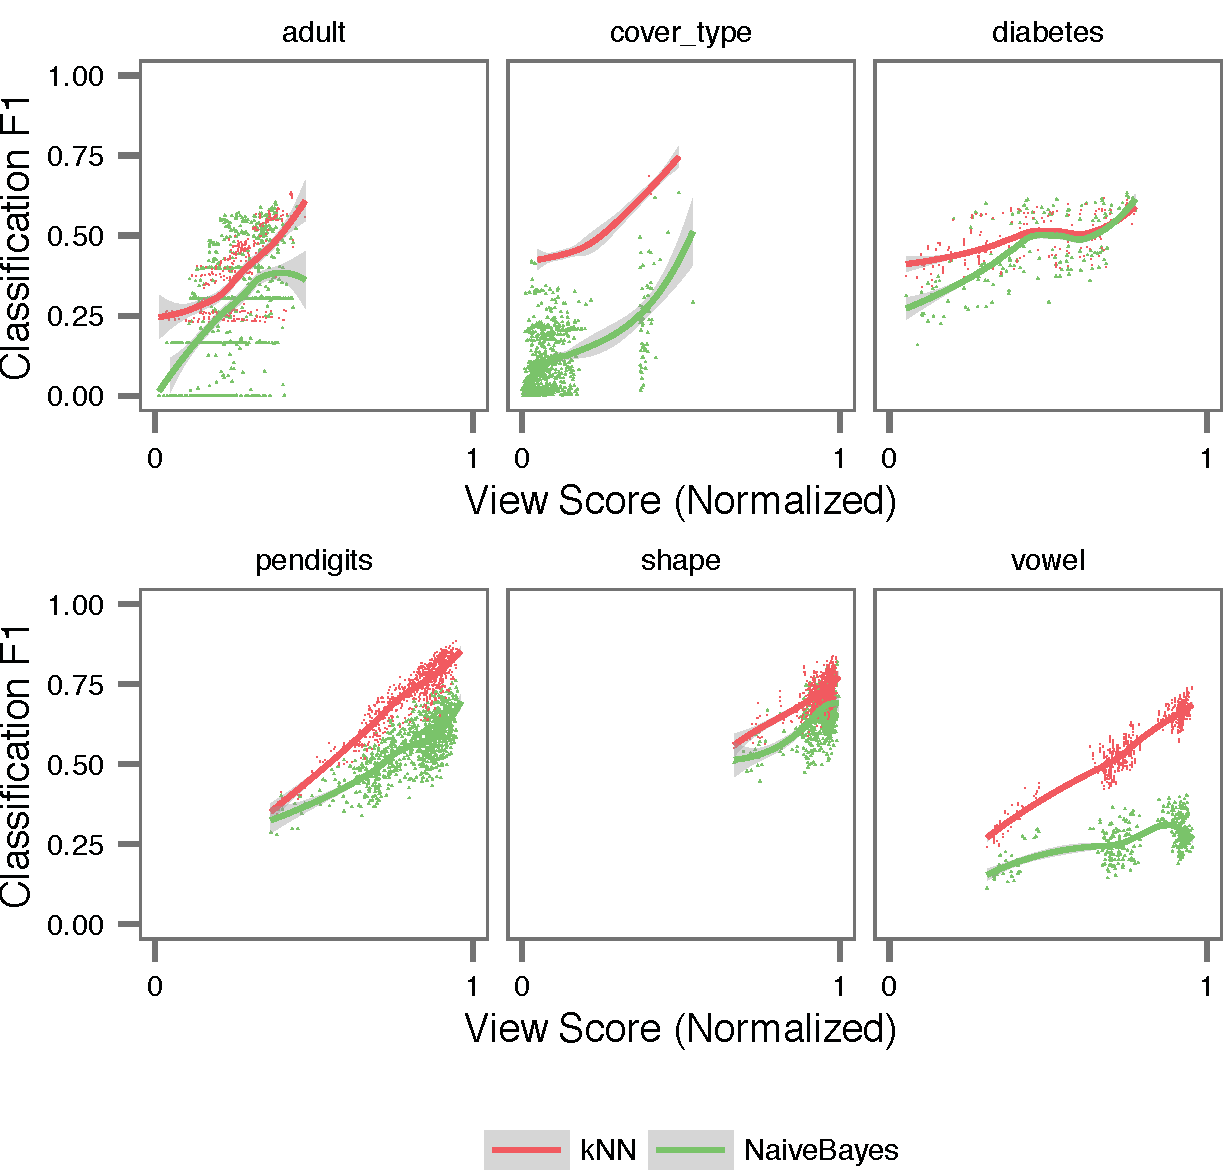
\includegraphics[width=\columnwidth]{plots/compare-strength-f1}
\caption{}
\label{pic:strength-vs-f1}
\end{figure}

\begin{figure*}[t!]
\centering
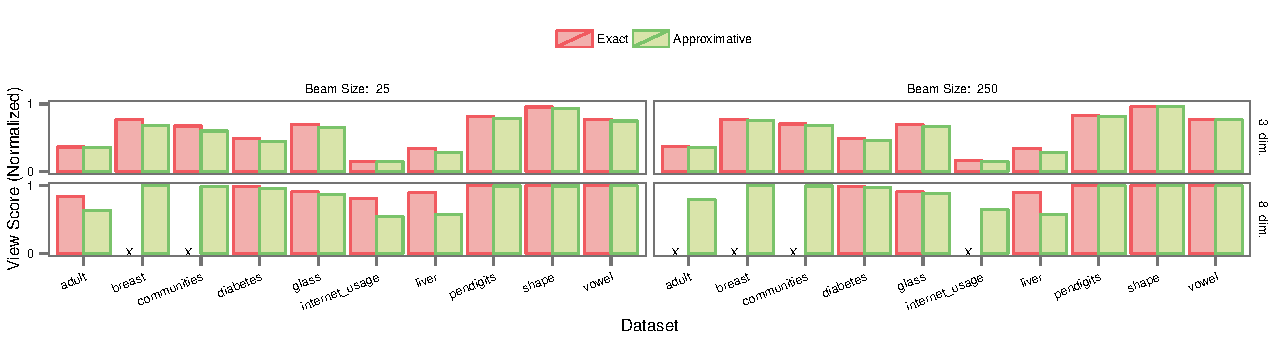
\includegraphics[width=2\columnwidth]{plots/column-select-score}
\caption{column-select-score}
\label{pic:column-select-score}
\end{figure*}

\begin{figure*}[t!]
\centering
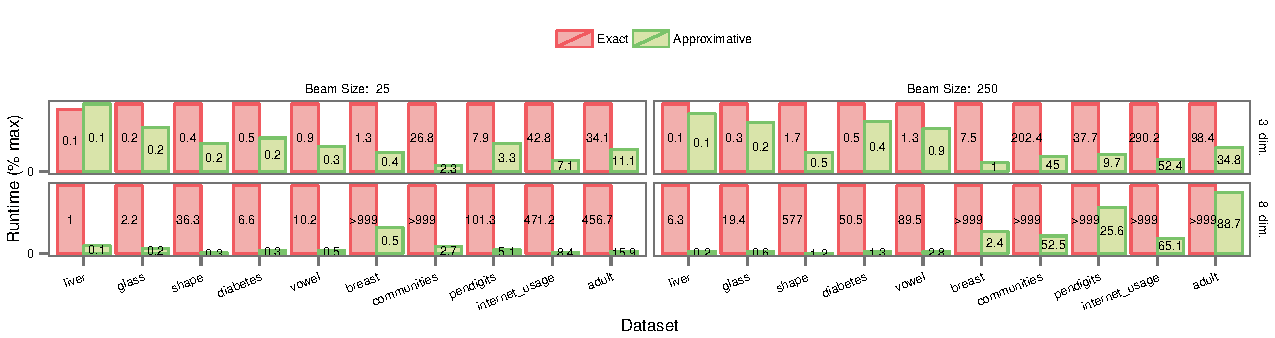
\includegraphics[width=2\columnwidth]{plots/column-select-time}
\caption{column-select-time}
\label{pic:column-select-time}
\end{figure*}
